\chapter{OPIS ROZWIĄZANIA}
\label{chapter:opis_rozwiazania}

\section{Architektura systemu}

System składa się z pięciu głównych komponentów: nadajników BLE (ang. \textit{BLE beacon}), aplikacji mobilnej, systemu Wit.ai, serwera oraz bazy danych. Grafikę przedstawiającą architekturę systemu można zobaczyć na rysunku \ref{fig:architecture}.

\begin{figure}[H]
    \centering
    \includesvg[width=\textwidth]{images/architecture.svg}
    \caption{Architektura systemu.}
    \label{fig:architecture}
\end{figure}

Aplikacja mobilna jest odpowiedzialna za odbieranie oraz przetwarzanie sygnału z nadajników. Jej zadaniem jest również interakcja z użytkownikiem i wysyłanie zapytań do serwera. Serwer przetwarza żądania użytkownika, wysyła zapytania do API (ang. \textit{Application Programming Interface}) serwisu Wit.ai, oraz komunikuje się z bazą danych. Baza danych przechowuje dane i modyfikuje lub udostępnia je na żadanie serwera. Komunikacja między aplikacją mobilną a serwerem odbywa się za pomocą protokołu HTTP. Serwer jest odpowiedzialny za przetwarzanie żądań użytkownika, a także za komunikację z bazą danych. Baza danych przechowuje dane o produktach, użytkownikach, koszykach, sklepach itp.

\section{Baza danych}

\subsection{Opis bazy danych}

Baza danych została zaimplementowana w PostgreSQL. Wybór tej bazy danych wynika z jej wszechstronności, wydajności oraz możliwości łatwego skalowania. 

PostgreSQL to obiektowo-relacyjny system zarządzania bazami danych (ang. ORDBMS \textit{Object-Relational Database Management System}), którego rozwój rozpoczął się już w 1977 roku. Jego korzenie sięgają projektu o nazwie Ingres, realizowanego na Uniwersytecie Kalifornijskim w Berkeley.
Uznawany jest za jeden z najbardziej zaawansowanych systemów baz danych o otwartym kodzie źródłowym na świecie. Oferuje wiele funkcji, które do tej pory były kojarzone głównie z komercyjnymi rozwiązaniami klasy enterprise. \cite{worsley2002practical}

Baza danych przechowuje informacje o produktach, użytkownikach, koszykach oraz sklepach. Schemat bazy danych przedstawia rysunek \ref{fig:database}.

Struktura bazy danych została zaprojektowana w sposób modularny, umożliwiając efektywne zarządzanie danymi dotyczącymi sklepów, użytkowników oraz produktów. Główną tabelą bazy danych jest tabela \textit{stores}, która przechowuje informacje o sklepach, takie jak nazwa, współrzędne geograficzne oraz miasto. Związek tej tabeli z tabelą \textit{sections} umożliwia podział sklepów na sekcje, które z kolei są przypisane do tabeli \textit{categories}, zawierającej dane o kategoriach produktów.

Produkty są przechowywane w tabeli \textit{products}, gdzie każdy rekord zawiera szczegóły takie jak nazwa, opis, cena, dostępność, ilość oraz jednostka miary, przechowywana w tabeli \textit{units}. Relacje między tabelami \textit{categories} i \textit{p}roducts pozwalają na przypisanie każdego produktu do konkretnej kategorii, co ułatwia organizację i wyszukiwanie danych.

Użytkownicy systemu są reprezentowani w tabeli \textit{users}, gdzie zapisywane są ich dane personalne, takie jak imię, nazwisko, adres e-mail oraz zaszyfrowane hasło. Każdy użytkownik może posiadać wiele koszyków zakupowych, co jest odzwierciedlone w tabeli \textit{carts}, przechowującej informacje o koszykach, takie jak data utworzenia i powiązanie z użytkownikiem. 
Szczegóły dotyczące zawartości koszyków są zapisane w tabeli \textit{cart\_items}, która łączy produkty z koszykami i zawiera informacje o liczbie sztuk danego produktu.

Relacje pomiędzy tabelami są realizowane za pomocą kluczy obcych, z zastosowaniem reguły ON DELETE CASCADE, co zapewnia integralność danych oraz automatyczne usuwanie powiązanych rekordów w przypadku usunięcia danych z tabel nadrzędnych. Taka organizacja umożliwia łatwe skalowanie bazy danych oraz wspiera utrzymanie spójności danych w systemie.

\begin{figure}[H]
    \includesvg[width=\textwidth]{images/database.svg}
    \caption{Schemat bazy danych.}
    \label{fig:database}
\end{figure}

\subsection{Szczegółowy opis tabel}

\subsubsection{Tabela stores}
\begin{itemize}
\item store\_id - SERIAL PRIMARY KEY: Unikalny identyfikator każdego sklepu.
\item store\_name - VARCHAR(255) NOT NULL: Nazwa sklepu.
\item latitude - VARCHAR(255) NOT NULL: Szerokość geograficzna określająca położenie sklepu.
\item longitude - VARCHAR(255) NOT NULL: Długość geograficzna określająca położenie sklepu.
\item city - VARCHAR(255) NOT NULL: Miasto, w którym znajduje się sklep.
\end{itemize}

\subsubsection{Tabela sections}
\begin{itemize}
\item section\_id - SERIAL PRIMARY KEY: Unikalny identyfikator sekcji sklepu.
\item section\_name - VARCHAR(255) NOT NULL: Nazwa sekcji w sklepie.
\item store\_id - INT REFERENCES stores(store\_id) ON DELETE CASCADE: Klucz obcy wskazujący sklep, do którego należy sekcja.
\end{itemize}

\subsubsection{Tabela categories}
\begin{itemize}
\item category\_id - SERIAL PRIMARY KEY: Unikalny identyfikator kategorii.
\item category\_name - VARCHAR(255) NOT NULL: Nazwa kategorii produktów.
\item section\_id - INT REFERENCES sections(section\_id) ON DELETE CASCADE: Klucz obcy wskazujący sekcję, do której przypisana jest kategoria.
\end{itemize}

\subsubsection{Tabela units}
\begin{itemize}
\item unit\_id - SERIAL PRIMARY KEY: Unikalny identyfikator jednostki miary.
\item unit\_name - VARCHAR(50) NOT NULL: Pełna nazwa jednostki miary (np. “kilogram”).
\item unit\_symbol - VARCHAR(10) NOT NULL: Skrót jednostki miary (np. “kg”).
\end{itemize}

\subsubsection{Tabela products}
\begin{itemize}
\item product\_id - SERIAL PRIMARY KEY: Unikalny identyfikator produktu.
\item name - VARCHAR(255) NOT NULL: Nazwa produktu.
\item description - TEXT: Opis produktu.
\item price - DECIMAL(10,2) NOT NULL: Cena produktu w formacie dziesiętnym (np. 123.45).
\item category\_id - INT REFERENCES categories(category\_id) ON DELETE CASCADE: Klucz obcy wskazujący kategorię, do której należy produkt.
\item availability - VARCHAR(50) NOT NULL: Status dostępności produktu (np. “w magazynie”).
\item amount - DECIMAL(10,2) NOT NULL: Ilość dostępna w magazynie.
\item unit\_id - INT REFERENCES units(unit\_id) ON DELETE CASCADE: Klucz obcy wskazujący jednostkę miary produktu.
\end{itemize}

\subsubsection{Tabela users}
\begin{itemize}
\item user\_id - SERIAL PRIMARY KEY: Unikalny identyfikator użytkownika.
\item email - VARCHAR(255) UNIQUE NOT NULL: Adres e-mail użytkownika.
\item password - VARCHAR(255) NOT NULL: Hasło użytkownika (w formie zaszyfrowanej).
\item first\_name - VARCHAR(50) NOT NULL: Imię użytkownika.
\item last\_name - VARCHAR(50) NOT NULL: Nazwisko użytkownika.
\end{itemize}

\subsubsection{Tabela carts}
\begin{itemize}
\item cart\_id - SERIAL PRIMARY KEY: Unikalny identyfikator koszyka.
\item user\_id - INT REFERENCES users(user\_id) ON DELETE CASCADE: Klucz obcy wskazujący użytkownika, do którego należy koszyk.
\item creation\_date - TIMESTAMP DEFAULT CURRENT\_TIMESTAMP: Data i czas utworzenia koszyka.
\end{itemize}

\subsubsection{Tabela cart\_items}
\begin{itemize}
\item cart\_item\_id - SERIAL PRIMARY KEY: Unikalny identyfikator pozycji w koszyku.
\item cart\_id - INT REFERENCES carts(cart\_id) ON DELETE CASCADE: Klucz obcy wskazujący koszyk, do którego należy pozycja.
\item product\_id - INT REFERENCES products(product\_id) ON DELETE CASCADE: Klucz obcy wskazujący produkt dodany do koszyka.
\item quantity - INT NOT NULL: Liczba sztuk danego produktu w koszyku.
\end{itemize}

\section{Interfejs użytkownika}

\subsection{Wykorzystane technologie}

\subsubsection{Wstęp}

Podczas budowy interfejsu użytkownika w projekcie wykorzsytano szereg nowoczesnych technologii oraz bibliotek, które wspólnie tworzą solidną i elastyczną podstawę dla aplikacji mobilnej. Postawiono na popularność rozwiązań i gotowych modułów oraz na możliwość zbudowania projektu na każdej platformie mobilnej. Poniżej przedstawiono szczegóły dotyczące użytych technologii oraz uzasadnienie ich wyboru.

\subsubsection{React Native}

React Native jest frameworkiem umożliwiającym tworzenie aplikacji mobilnych na platformy iOS oraz Android przy użyciu jednego kodu w JavaScript lub TypeScript. Dzięki React Native zredukowaliśmy czas i koszty produkcji aplikacji, jednocześnie zachowując natywną wydajność. Co więcej nauka React Native jest stosunkowo prosta, dla osób które pisały aplikacje przeglądarkowe we frameworku \textit{React}.

\subsubsection{Expo}

Expo to platforma usprawniająca rozwój aplikacji w React Native. Zapewnia bogaty zestaw narzędzi, takich jak menedżer pakietów, biblioteki gotowe do użycia i uproszczony proces wdrażania. Wybór Expo pozwolił na przyspieszenie rozwoju aplikacji oraz zwinne uruchamianie jej w trybie developerskim na urządzeniach mobilnych.

\subsubsection{TypeScript}

TypeScript to rozszerzenie \textit{JavaScriptu}, które dodaje statyczne typowanie. Dzięki niemu kod aplikacji jest bardziej przejrzysty i mniej podatny na błędy. TypeScript wspomaga skalowalność projektu oraz ułatwia współpracę między programistami. Dzieki wykorzystaniu tego języka zwiększono jakość kodu oraz uniknięto wielu potencjhnych błędów, wynikających z niepoprawnego typowania zmiennych. 

\subsubsection{Kluczowe biblioteki}

\begin{itemize}
    \item \textbf{expo-speech-recognition} - Umożliwia rozpoznawanie mowy użytkownika. Użycie tej technologii pozwala na obsługę aplikacji za pomocą poleceń głosowych, co znacząco zwiększa jej dostępność, szczególnie dla osób z trudnościami w obsłudze interfejsu dotykowego. Zastosowanie jej jest kluczowe w udostępnieniu aplikacji dla niewidomych i odbieraniu ich komend głosowych.
    \item \textbf{expo-speech} - Biblioteka ta pozwala na syntezę mowy w aplikacjach React Native. Dzięki niej aplikacja może przekazywać informacje użytkownikowi za pomocą komunikatów głosowych, co daje szanse osobom niepełnosprawnym na korzystanie z aplikacji.
    \item \textbf{react-native-ble-plx} - Obsługuje komunikację Bluetooth Low Energy (BLE). Została wybrana ze względu na swoją popularność oraz możliwość integracji z natywnymi modułami Bluetooth, co jest niezbędne w przypadku funkcji wymagających interakcji z urządzeniami zewnętrznymi.
    \item \textbf{expo-secure-store} - Użycie jej umożliwia bezpieczne przechowywanie danych, takich jak tokeny sesji lub dane uwierzytelniające. Dzięki integracji z Expo oraz wsparciu dla mechanizmów natywnych wybór tej biblioteki zapewnia wysoki poziom ochrony danych użytkownika i pozwala na łatwy dostęp do charakterystycznych zmiennych globalnych.
    \item \textbf{react-native-svg} - Obsługuje grafiki wektorowe w formacie SVG w aplikacjach React Native. Umożliwia tworzenie dynamicznych, skalowalnych elementów graficznych, takich jak wykresy, ikony czy kody QR, co czyni ją idealnym wyborem w aplikacjach wymagających dużej precyzji graficznej. W kontekście naszej aplikacji pozwala na generowanie map sklepów w prosty sposób.
    \item \textbf{react-native-qrcode-svg} - Odpowiedzialna za generowanie kodów QR w aplikacjach React Native. Została użyta w projekcie do generowania kodów QR na podstawie produktów w koszyku, co pozwala użytkownikowi na łatwe zeskanowanie i zrealizowanie transakcji w sklepie.
    \item \textbf{react-native-maps} - Umożliwia wyświetlanie map w aplikacjach React Native. W projekcie odegrała kluczową rolę w tworzeniu widoku mapy sklepu, pozwalając użytkownikowi na wybór najbliższego sklepu z listy dostępnych lokacji, a także umożliwiając wyświetlanie jego lokalizacji na mapie.
\end{itemize}

\section{Serwer aplikacji}
Serwer jest odpowiedzialny za przetwarzanie żądań użytkownika, a także za komunikację z bazą danych. Został zaimplementowany w języku JavaScript przy użyciu platformy Node.js oraz struktury (ang. \textit{framework}) Express.js. Node.js pozwala na uruchamianie JavaScript po stronie serwera, co umożliwia tworzenie wydajnych i skalowalnych aplikacji. Express.js, będący minimalistycznym frameworkiem działającym na Node.js, upraszcza proces budowy aplikacji internetowych. Serwer nasłuchuje na zapytania HTTP, przetwarza je i zwraca odpowiedź, a do komunikacji z bazą danych PostgreSQL wykorzystuje odpowiednie moduły Node.js.


\subsection{JavaScript}
JavaScript jest podstawowym językiem programowania w sieci Web. Zdecydowana większość współczesnych stron internetowych wykorzystuje JavaScript, a wszystkie nowoczesne przeglądarki internetowe — zarówno na komputerach stacjonarnych, konsolach do gier, tabletach, jak i smartfonach — posiadają wbudowane interpretery tego języka. Dzięki temu JavaScript stał się najbardziej wszechobecnym językiem programowania w historii. Wraz z HTML, odpowiadającym za treść stron, oraz CSS, definiującym ich wygląd, JavaScript stanowi podstawowy zestaw technologii, które każdy programista webowy musi opanować, aby określać zachowanie stron internetowych. \cite{flanagan2011javascript}


\subsection{Node.js}
Node.js umożliwia programistom wykorzystywanie JavaScript po stronie serwera, co pozwala na tworzenie aplikacji full-stack przy użyciu jednego języka. Dzięki architekturze wspierającej asynchroniczne i nieblokujące operacje I/O świetnie sprawdza się w obsłudze wielu jednoczesnych połączeń. \cite{peters2017building}

Dzięki architekturze opartej na zdarzeniach oraz jednowątkowemu modelowi działania, Node.js idealnie nadaje się do tworzenia aplikacji czasu rzeczywistego, takich jak czaty, narzędzia do współpracy czy usługi streamingowe. \cite{peters2017building}

\subsection{Express.js}
Express.js to minimalistyczny framework dla Node.js, który pozwala na szybkie tworzenie aplikacji internetowych. Dzięki swojej prostocie i elastyczności jest jednym z najpopularniejszych frameworków dla Node.js.

Framework Express.js umożliwia dynamiczny routing, pozwalając programistom na definiowanie wzorców URL i przypisywanie ich do określonej logiki aplikacji. Taka elastyczność ułatwia zarządzanie złożonymi strukturami aplikacji poprzez wiązanie punktów końcowych z odpowiednimi kontrolerami. \cite{peters2017building}

\section{System nawigacji}

\subsection{Wprowadzenie do systemu nawigacji}
Celem systemu nawigacji jest dostarczenie użytkownikowi (klientowi sklepu) intuicyjnych i precyzyjnych wskazówek pomagających w odnalezieniu poszukiwanych produktów wewnątrz budynku. System łączy w sobie dokładne modelowanie sklepu w formie grafu, pozycjonowanie użytkownika z wykorzystaniem technologii BLE, a także efektywne algorytmy znajdowania i optymalizacji tras. Założeniem jest, aby klient mógł szybko i sprawnie dotrzeć do wszystkich potrzebnych mu produktów, minimalizując czas i dystans pokonany w obrębie sklepu.

Przedstawiona koncepcja opiera się na kilku kluczowych elementach. Po pierwsze, środowisko sklepu modelowane jest jako graf, którego wierzchołkami są sekcje sklepu. Po drugie, użytkownik jest lokalizowany wzdłuż alejki w sposób jednoosiowy, co upraszcza problem pozycjonowania. Po trzecie, trasa wyznaczana jest na podstawie listy docelowych sekcji, a następnie optymalizowana, również w trakcie poruszania się klienta po sklepie. Całość tworzy spójny, interaktywny system nawigacji działający w czasie rzeczywistym.

\subsection{Opis środowiska i infrastruktury sklepu}

\subsubsection{Charakterystyka sklepu i układ alejek}
Rozważany sklep można przedstawić jako pomieszczenie z kilkoma długimi, równoległymi alejkami, połączonymi na końcach przejściami poprzecznymi. Wzdłuż alejek rozmieszczone są regały z towarami. Przestrzeń ta jest zorganizowana w taki sposób, aby klient mógł łatwo przemieszczać się po regularnych ścieżkach, bez konieczności kluczenia w labiryncie nieuporządkowanych półek.

Na ogół alejki mają podobną długość, a przejścia między nimi są umiejscowione w ustalonych, regularnych miejscach. To znacząco obniża złożoność problmu nawigacji.
\subsubsection{Lokalizacja i oznaczanie sekcji w alejkach}
Każda alejka dzielona jest na mniejsze odcinki, zwane sekcjami, z których każda zawiera określoną grupę produktów. Sekcje są numerowane wzdłuż alejki, np. od 1.0 do 8.0, a dodatkowo można wyróżnić połówkowe wartości (1.5, 2.5, ...) w celu precyzyjniejszej lokalizacji. Identyfikatory sekcji są używane do powiązania konkretnych produktów z miejscem w sklepie, w którym się znajdują. Dzięki temu, gdy klient określi listę zakupów, system może przełożyć ją na zbiór sekcji do odwiedzenia.

\subsection{Modelowanie przestrzeni sklepu jako graf}

\subsubsection{Definicja wierzchołków i krawędzi grafu sklepu}
W modelu grafowym każda sekcja to wierzchołek grafu. Między wierzchołkami istnieją krawędzie reprezentujące możliwość przejścia z jednej sekcji do drugiej. Wagi krawędzi odpowiadają fizycznym odległościom - często są one identyczne w obrębie alejki.

Zwykle alejka jest reprezentowana jako ciąg wierzchołków połączonych liniowo. Jeśli istnieją przejścia poprzeczne między alejkami, to w grafie pojawiają się krawędzie łączące wierzchołki reprezentujące sekcje różnych alejek. Dzięki temu graf odzwierciedla fizyczną strukturę sklepu i umożliwia stosowanie standardowych algorytmów grafowych.

\subsubsection{Reprezentacja sekcji jako węzłów grafu}
Każda sekcja ma przypisany numer i stanowi osobny węzeł w grafie. W przypadku alejki dzielonej na 8 sekcji, graf może zawierać wierzchołki 1, 2, 3, ... 8, połączone krawędziami reprezentującymi kolejne odcinki alejki. Jeśli do jednej z sekcji można dojść z sąsiedniej alejki, w grafie pojawia się dodatkowa krawędź.

Taka reprezentacja pozwala łatwo rozszerzać i modyfikować układ sklepu. Dodanie nowej sekcji lub zmiana odległości pomiędzy sekcjami sprowadza się do manipulacji wierzchołkami i krawędziami w grafie.

\subsubsection{Ilustracje graficzne: rzut sklepu i odpowiadający mu graf}

\begin{figure}[H]
\centering
\begin{minipage}{0.45\linewidth}
\centering
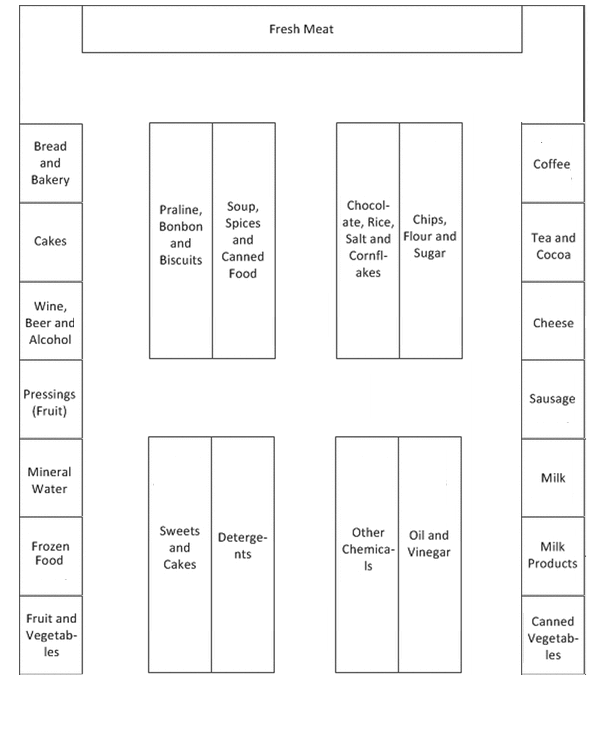
\includegraphics[width=\textwidth]{images/rzut_sklepu.png}
\caption{Rzut przykładowego sklepu (źródło: \cite{woeginger2016}).}
\label{fig:rzut_sklepu}
\end{minipage}
\hfill
\begin{minipage}{0.45\linewidth}
\centering
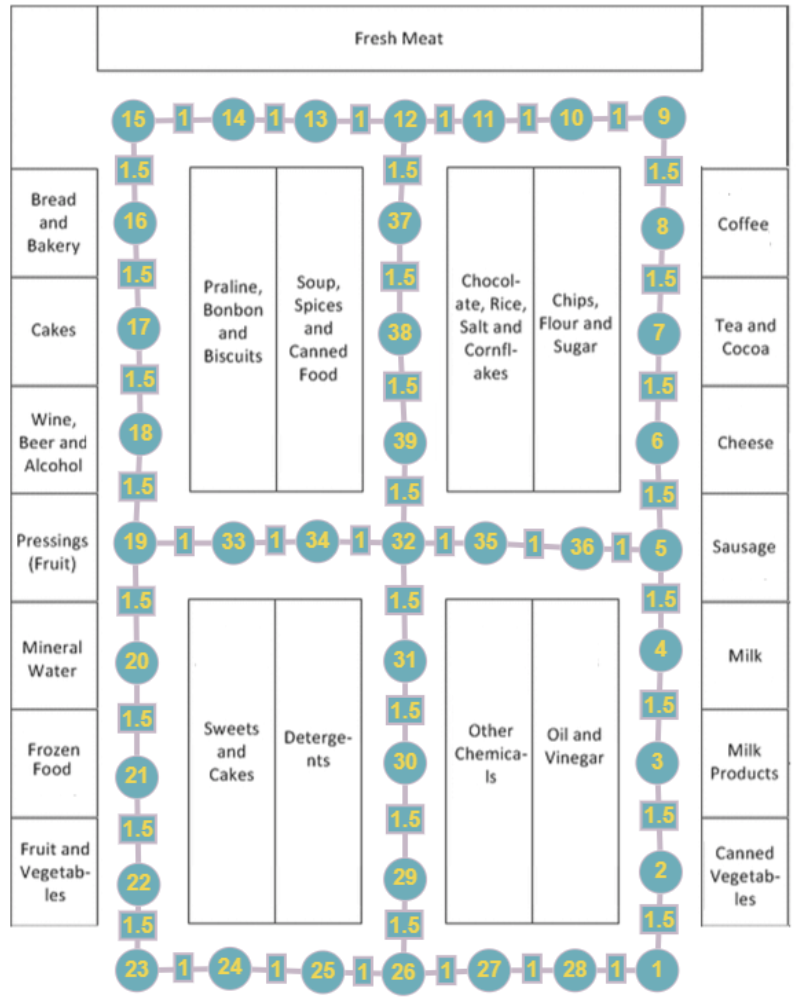
\includegraphics[width=\textwidth]{images/graf_sklepu.png}
\caption{Zmapowanie rzutu sklepu na graf.}
\label{fig:graf_sklepu}
\end{minipage}
\end{figure}


\subsection{Pozycjonowanie użytkownika – podejścia, algorytmy i optymalizacje}

\subsubsection{Wcześniejsze próby i porzucone podejścia}
Przed opracowaniem finalnego rozwiązania jednoosiowego pozycjonowania, przeprowadzono szereg eksperymentów z innymi technikami. Niestety, z różnych powodów nie spełniły one wymagań co do dokładności, stabilności i responsywności systemu.

\paragraph{Fingerprinting}
Pierwszą z prób było zastosowanie techniki fingerprintingu. Polega ona na tworzeniu szczegółowej mapy wartości RSSI dla różnych punktów w sklepie, a następnie porównywaniu aktualnych pomiarów z tą mapą referencyjną. Mimo początkowych nadziei, fingerprinting okazał się bardzo niestabilny. Szumy sygnałowe były na tyle silne, że trudno było uzyskać powtarzalne i spójne wyniki. W efekcie, pozycjonowanie było nieprecyzyjne, a różnice nawet kilku metrów zdarzały się często. Taka niedokładność sprawiała, że metoda była bezużyteczna w praktyce i została porzucona.

\paragraph{Dodatkowe filtracje i predykcje (x,y)}
Kolejną próbą było rozbudowanie filtracji Kalmana o model dwuwymiarowy (x, y), aby nie tylko wygładzać RSSI, ale też predykować ruch użytkownika w pełnej płaszczyźnie sklepu. Ten pomysł faktycznie zwiększył stabilność pomiarów i ich przewidywalność, ale odbyło się to kosztem wydajności i responsywności. System stał się mocno spowolniony, a długotrwała predykcja powodowała, że reagował z opóźnieniem na faktyczne zmiany położenia użytkownika, „uparcie” trzymając się wyuczonego modelu. W praktyce użytkownik poruszał się, a system nie nadążał z aktualizacją jego pozycji. Ostatecznie uznano, że takie podejście jest nieefektywne i zrezygnowano z niego.

\paragraph{Trilateracja}
Próbowano również wykorzystać klasyczną trilaterację, polegającą na wyznaczaniu pozycji w oparciu o odległości do trzech nadajników rozmieszczonych w znanych punktach sklepu. Niestety, w środowisku sklepowym odbicia, tłumienia i interferencje sygnału powodowały, że obliczenia były bardzo niestabilne. Natomiast głównym problemem była znaczna niedokładność wyników. Nie udało się osiągnąć satysfakcjonującej jakości, więc trilateracja również została zarzucona.

\paragraph{Metoda centroidów}
Kolejnym testowanym sposobem była metoda centroidów, w której pozycję użytkownika określa się jako środek ciężkości położeń najbliższych nadajników. Chociaż podejście jest proste i szybkie, w testach okazało się, że wyniki były niezwykle niestabilne. Nawet przy braku ruchu użytkownika, estymowana pozycja nie była stabilna. Metoda nie zapewniała więc żadnej użytecznej stabilności.

\subsubsection{Wprowadzenie do jednoosiowego pozycjonowania w alejce}
Tradycyjne systemy pozycjonowania wewnętrznego często próbują określić pełną pozycję (x, y) użytkownika wewnątrz budynku. W naszym rozwiązaniu upraszczamy ten problem, skupiając się wyłącznie na jednym wymiarze – pozycji wzdłuż alejki. Obserwacja jest taka, że klient porusza się głównie wzdłuż linii alejek, a dostęp do towarów z jednej strony jest na tyle ograniczony, że nie ma potrzeby znać dokładnego położenia w dwóch wymiarach.

Dzięki temu zamiast skomplikowanych algorytmów dwuwymiarowych, stosujemy jednoosiowe pozycjonowanie, traktując alejkę jak oś liczbową, na której poszczególne sekcje i ich granice są reprezentowane przez wartości liczbowe.
\subsubsection{Rozmieszczenie nadajników BLE i koncepcja punktów odniesienia}
Do pozycjonowania wykorzystujemy sieć nadajników BLE (beaconów) rozmieszczonych wzdłuż alejki w stałych odstępach. Podstawowe punkty odniesienia to całkowite wartości odpowiadające początkom sekcji (np. 1.0, 2.0, 3.0, ...), zaś dodatkowe nadajniki umieszczone są w połowie sekcji (np. 1.5, 2.5, 3.5, ...) dla uzyskania większej precyzji.

Takie zagęszczenie punktów odniesienia sprawia, że pomiar sygnału z kilku nadajników jednocześnie pozwala nie tylko określić, w której sekcji jest klient, ale również dokładniejsze położenie w jej obrębie. Zamiast wskazać sekcję nr 2, system może ustalić, że użytkownik jest np. w 37% jej długości.
\subsubsection{Szacowanie odległości na podstawie RSSI}
Podstawą pozycjonowania jest pomiar siły sygnału RSSI emitowanego przez nadajniki BLE. RSSI maleje wraz ze wzrostem odległości, co pozwala na estymację dystansu. Przyjmując prosty model logarytmiczny, można odwrócić zależność i wyliczyć przybliżoną odległość \( d \) od nadajnika na podstawie zmierzonej wartości RSSI.

\[
\text{RSSI}(d) = \text{RSSI}_{\text{ref}} - 10 \cdot n \cdot \log_{10}(d) \quad \Rightarrow \quad d = 10^{\frac{\text{RSSI}_{\text{ref}} - \text{RSSI}(d)}{10 \cdot n}}
\]

Parametry \(\text{RSSI}_{\text{ref}}\) oraz \( n \) (wykładnik strat propagacyjnych) dobiera się doświadczalnie. Tak uzyskane wartości odległości są jednak zaszumione, więc przed wykorzystaniem ich do obliczenia pozycji konieczne jest wygładzanie pomiarów.

\subsubsection{Zastosowanie filtru Kalmana do stabilizacji pomiarów}
Aby zredukować szum i fluktuacje w pomiarach RSSI, stosujemy filtr Kalmana. Pozwala on łączyć aktualne pomiary z predykcją stanu, co skutkuje płynniejszym i stabilniejszym odczytem odległości.

Filtr Kalmana iteracyjnie:
\begin{itemize}
    \item Przewiduje wartość RSSI na podstawie poprzedniej estymacji.
    \item Koryguje przewidywanie, uwzględniając nowy pomiar.
\end{itemize}

Dzięki temu wartości odległości uzyskane z RSSI są mniej podatne na chwilowe zaburzenia, co przekłada się na dokładniejsze pozycjonowanie.

\subsubsection{Obliczanie pozycji użytkownika w czasie rzeczywistym}
Po przefiltrowaniu odległości do nadajników obliczamy pozycję klienta jako ważoną średnią ich znanych położeń. Wagi definiujemy odwrotnie proporcjonalnie do kwadratu odległości:

\[
w_i = \frac{1}{d_i^2}, \quad \hat{P} = \frac{\sum_i (w_i \cdot p_i)}{\sum_i w_i}
\]

gdzie \( p_i \) to pozycja nadajnika, a \( d_i \) obliczona odległość. W ten sposób nadajniki najbliższe mają większy wpływ na wynik, zapewniając bardziej precyzyjne określenie miejsca użytkownika.

\subsubsection{Interpretacja pozycji – przejście od sekcji dyskretnych do wartości rzeczywistych}
Uzyskana pozycja \(\hat{P}\) może być liczbą zmiennoprzecinkową, np. 2.37486, co oznacza, że użytkownik znajduje się pomiędzy początkami sekcji 2.0 i 3.0, bliżej końca sekcji 2. Takie ciągłe podejście zwiększa czytelność i precyzję, umożliwiając wyświetlenie użytkownikowi płynnie przesuwającej się kropki na mapie alejki.

\subsection{Wyznaczanie ścieżki i wykorzystanie pozycji użytkownika}

\subsubsection{Mapowanie listy produktów na sekcje}
Pierwszym krokiem do wyznaczenia trasy jest przełożenie listy zakupów na konkretne sekcje sklepu. Każdy produkt w bazie danych jest przypisany do określonej sekcji. Gdy użytkownik poda listę interesujących go towarów, system odczytuje te informacje i tworzy zbiór docelowych sekcji, które należy odwiedzić.

Na przykład, jeśli produkty to \{mleko, jogurt, masło\}, a wszystkie znajdują się w sekcji 7, docelowy zestaw to \{7\}. Jeśli produkty są rozproszone w różnych częściach sklepu, np. sekcja 3, 7 i 10, to system musi wziąć pod uwagę wizytę w każdej z tych sekcji.

\subsubsection{Algorytmy znajdowania najkrótszych ścieżek (Dijkstra, 2-opt i inne)}
Wyznaczenie optymalnej trasy, która obejmuje przejście przez wszystkie wybrane sekcje sklepu (wynikające z listy zakupów), jest wyzwaniem zbliżonym do problemu komiwojażera. Mimo to, w naszym podejściu stosujemy prostszy i bardziej praktyczny algorytm wieloetapowy, oparty na połączeniu metody znajdowania najkrótszych ścieżek (Dijkstry) oraz heurystyki optymalizacyjnej (2-opt).

\paragraph{Krok 1: Iteracyjne wyznaczanie trasy przy użyciu algorytmu Dijkstry}
Na początku dysponujemy listą sekcji, które użytkownik musi odwiedzić, oraz jego bieżącą pozycją startową w sklepie. Proces budowania trasy przebiega iteracyjnie:
\begin{enumerate}
    \item Uruchamiamy algorytm Dijkstry, biorąc za punkt startowy aktualną pozycję użytkownika. Dijkstra oblicza najkrótsze ścieżki do wszystkich wierzchołków (sekcji) w grafie.
    \item Spośród jeszcze nieodwiedzonych docelowych sekcji wybieramy tę, która jest najbliższa (czyli ma najmniejszy dystans wg Dijkstry). W ten sposób dokonujemy „chciwego” (\emph{greedy}) wyboru kolejnej sekcji do odwiedzenia.
    \item Odtwarzamy ścieżkę do wybranej sekcji (za pomocą informacji uzyskanych z algorytmu Dijkstry) i dołączamy ją do naszej powstającej trasy.
    \item Aktualizujemy pozycję startową na tę właśnie odwiedzoną sekcję i usuwamy ją ze zbioru pozostałych do odwiedzenia.
\end{enumerate}

Te kroki powtarzane są do momentu, aż odwiedzimy wszystkie sekcje z listy zakupów. W efekcie otrzymujemy trasę, która zawiera wszystkie wymagane punkty, choć kolejność ich odwiedzania została ustalona w sposób chciwy (zawsze wybierając najbliższy jeszcze nieodwiedzony cel).

\paragraph{Krok 2: Heurystyczna optymalizacja trasy (2-opt)}
Otrzymana w powyższy sposób trasa może nie być globalnie optymalna, jednak stanowi dobrą bazę wyjściową do dalszej optymalizacji. W kolejnym etapie stosujemy heurystykę 2-opt, polegającą na iteracyjnym sprawdzaniu, czy odwrócenie fragmentów trasy (zamiana kolejności przejść między kilkoma punktami) nie skróci jej całkowitej długości. Jeśli taka zmiana jest korzystna, trasa zostaje zaktualizowana. Proces ten jest powtarzany, dopóki nie można już znaleźć dalszej poprawy.

\paragraph{Zalety takiego podejścia}
Połączenie algorytmu Dijkstry i heurystyki 2-opt oferuje kilka korzyści:
\begin{itemize}
    \item Uproszczenie problemu: Zamiast bezpośrednio rozwiązywać trudne zagadnienie komiwojażera, rozbijamy je na sekwencję prostszych podproblemów wyboru najbliższego celu.
    \item Efektywność obliczeniowa: Dijkstra pozwala szybko i dokładnie ustalić najkrótsze ścieżki do kolejnych celów, a chciwy wybór upraszcza proces generowania trasy.
    \item Poprawa jakości wyniku: Zastosowanie 2-opt pozwala skrócić wstępnie znalezioną trasę, zbliżając ją do lokalnego optimum bez konieczności kosztownego przeszukiwania wszystkich możliwych permutacji.
\end{itemize}

W ten sposób system nawigacji potrafi sprawnie poprowadzić użytkownika przez cały sklep, zachowując równowagę pomiędzy prostotą obliczeń, a jakością uzyskanej trasy.

\subsection{Integracja pozycjonowania i trasowania}

\subsubsection{Dynamiczne dostosowywanie trasy do pozycji użytkownika}
Integracja informacji o bieżącej pozycji użytkownika z wyznaczoną trasą pozwala na elastyczne reagowanie na zmiany w środowisku sklepu i preferencjach klienta. Jeżeli użytkownik w trakcie zakupów zboczy z wyznaczonej ścieżki, pominie którąś z zaplanowanych sekcji lub zdecyduje się na odwiedzenie innego produktu, system może w dowolnym momencie ponownie wyznaczyć trasę, uwzględniając nową pozycję oraz aktualną listę celów.

Takie podejście sprawia, że nawigacja staje się w pełni interaktywna i dopasowana do bieżących potrzeb użytkownika. Aktualizacja trasy zachodzi cyklicznie (w stałych odstępach czasu) lub w reakcji na znaczne zmiany położenia klienta bądź modyfikacje listy produktów. Dzięki temu klienci otrzymują wskazówki oparte na aktualnym kontekście, co zwiększa komfort zakupów oraz poprawia efektywność poruszania się po sklepie.

\subsubsection{Wykorzystanie informacji o ruchu użytkownika do korekcji błędów pozycjonowania}
Informacje o tym, jak użytkownik się przemieszcza, mogą pomóc w poprawie dokładności pozycjonowania. Jeśli pomiar RSSI lub filtr Kalmana zasugerują nagły skok pozycji w nielogicznym kierunku, system może sprawdzić, czy na grafie istnieje taka możliwość ruchu. Jeżeli nie, skok można uznać za błąd pomiaru i skorygować pozycję użytkownika.

W ten sposób trasa i pozycjonowanie wzajemnie się wspierają. Trasa nadaje kontekst położeniu klienta, a położenie klienta pomaga wykrywać anomalie i błędy w pomiarach. W efekcie system staje się bardziej odporny na zakłócenia środowiskowe i zapewnia użytkownikowi lepsze, bardziej spójne doświadczenie nawigacyjne.

\subsection{Podsumowanie}
Przedstawiony system nawigacji wewnątrz sklepu integruje różnorodne elementy:
\begin{itemize}
    \item Modelowanie przestrzeni sklepu jako grafu, ułatwiające wyznaczanie ścieżek.
    \item Jednoosiowe pozycjonowanie użytkownika z wykorzystaniem nadajników BLE i filtracji pomiarów filtrem Kalmana, zapewniające stabilne i precyzyjne określenie miejsca w alejce.
    \item Algorytmy wyznaczania i optymalizacji ścieżek (Dijkstra, 2-opt) oraz mechanizmy dynamicznego dostosowywania trasy do aktualnej pozycji i zachowania użytkownika.
    \item Integracja pozycjonowania i trasowania, pozwalająca wykrywać i korygować ewentualne błędy pomiarowe, a także elastycznie reagować na zmiany w środowisku sklepu.
\end{itemize}
